\documentclass[pdf, 9pt,intlimits, unicode]{beamer}

% If you have more than three sections or more than three subsections in at least one section,
% you might want to use the [compress] switch. In this case, only the current (sub-) section
% is displayed in the header and not the full overview.
\mode<presentation>
{
	\usetheme[numbers, totalnumbers, minimal]{Statmod}
	
	\setbeamercovered{transparent}
	% or whatever (possibly just delete it)
}
\usepackage[utf8]{inputenc} %

\usepackage[T2A]{fontenc} %
\usepackage[russian]{babel} %
\usepackage{subcaption}

\usepackage{makecell}
\usepackage{amsmath}
\usepackage{amsfonts}
\usepackage{bm}
\usepackage{graphicx}
\usepackage{multicol}
%\usepackage[usenames]{color}
\usepackage{colortbl}
\usepackage{euscript}
\usepackage{booktabs}
\usepackage{longtable}
\usepackage{multirow}
\usepackage{pdflscape}
% Использовать полужирное начертание для векторов
\let\vec=\mathbf

\DeclareMathOperator{\mathspan}{span}
\DeclareMathOperator{\mathdim}{dim}
\DeclareMathOperator{\rank}{rank}
\DeclareMathOperator{\diag}{diag}
\newcommand\eqdef{\mathrel{\stackrel{\makebox[0pt]{\mbox{\normalfont\tiny def}}}{=}}}

\title[Обнаружение разладки с помощью метода SSA]{«Обнаружение разладки с помощью метода SSA»}
\author{Кононыхин Иван Александрович, группа 20.М03-мм}

\subtitle{Презентация ВКР}
%\logo{}
\institute[СПбГУ]{Санкт-Петербургский государственный университет \\
	Математико-механический факультет \\
	Кафедра статистического моделирования \\
	\vspace{0.4cm}
	Научный руководитель: к.ф.-м.н., доцент Голяндина Н.Э. \\
	Рецензент: Лектор, Университет Кардиффа (Великобритания), Пепелышев А.Н. \\
	\vspace{0.3cm}
}
\date{
	Санкт-Петербург\\
	2022г.
}
%\setbeameroption{show notes}
\begin{document}
	\begin{frame}
		\maketitle
	\end{frame}

	\begin{frame}
		\frametitle{Введение: постановка задачи}
		\textbf{Однородный} ряд --- ряд с постоянной структурой. \textbf{Разладка} --- нарушение однородности ряда. 
		
		\bigskip
		{\color{blue} Задача обнаружения разладки:}
		Определить момент изменения структуры ряда. Структура --- подпространство сигнала.
		
		\bigskip
		{\color{blue} Метод:}
		Превышение порога функцией обнаружения неоднородности, основанной на разнице структур скользящих отрезков ряда.
		
		\bigskip
		
		{\color{blue} Временной ряд:} 
		
		$ F_N=(f_1, \dots, f_{N}) $, где $f_n = 
		\begin{cases}
			C_1\sin(2\pi\omega_1n + \phi_1),& n < Q, \\
			C_2\sin(2\pi\omega_2n + \phi_2),& n \geq Q,
		\end{cases}$
		
		$ Q $ --- неизвестный момент возмущения.
		
		\bigskip
		{\color{blue} Цель работы:} 
		Создание системы, которая:
		\begin{enumerate}
			\item Определяет разладку, заданную изменением частоты.
			\item Автоматически выбирает порог срабатывания.
			\item Сообщает о моменте возмущения с заданным значением максимально допустимого запаздывания.
		\end{enumerate}
	\end{frame}

	\begin{frame}
		\frametitle{Введение: обозначения}	
		{\color{blue} Параметры:} $ L $, $ B $, $ T $, $ r = 2 $.
		\begin{center}
			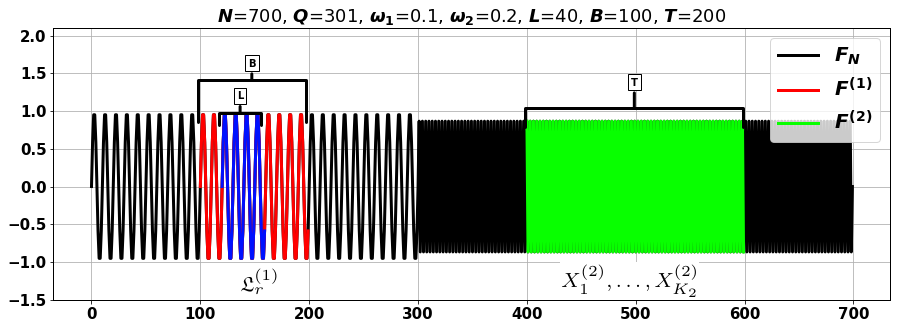
\includegraphics[width=\linewidth]{imgs/designations}
		\end{center}
%		\begin{itemize}
%			\item $ \mathfrak{L}_r^{(1)} \eqdef \mathspan(\{U_1^{(1)}, U_2^{(1)}\}) $.
%		\end{itemize}

		\bigskip
		
		{\color{blue} Индекс неоднородности} (Golyandina, Nekrutkin, Zhigljavsky. Analysis of Time Series Structure. 2001):
		\small{
			$$ g(F^{(1)}; F^{(2)}) = \frac{\sum\limits_{l=1}^{K_2}\mathrm{dist}^2(X_l^{(2)}, \mathfrak{L}_r^{(1)})}{\sum\limits_{l=1}^{K_2}\|X_l^{(2)}\|^2}. $$
		}
	\end{frame}

	\begin{frame}
		\bigskip
		\frametitle{Введение: инструменты поиска неоднородности}
		\begin{multicols}{2}
			
			\begin{figure}
				\center
				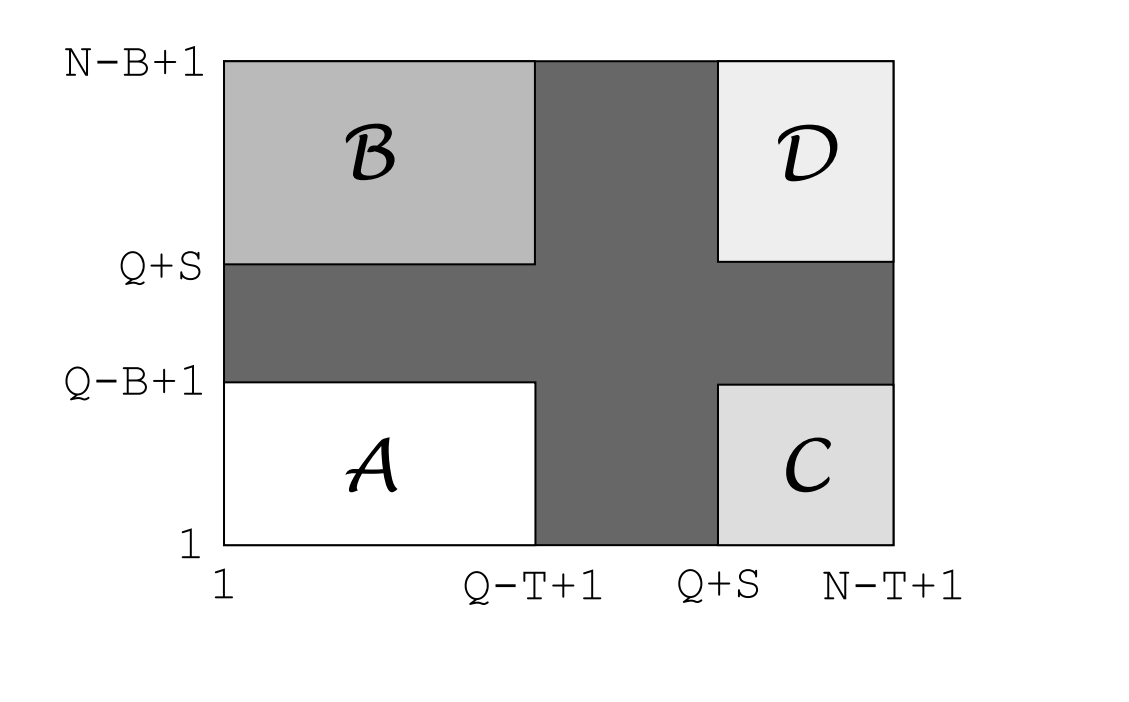
\includegraphics[width=\linewidth, height=0.8\linewidth]{imgs/H-matrix}\caption{Матрица неоднородности}\par 
			\end{figure}
			\begin{figure} 
				\center
				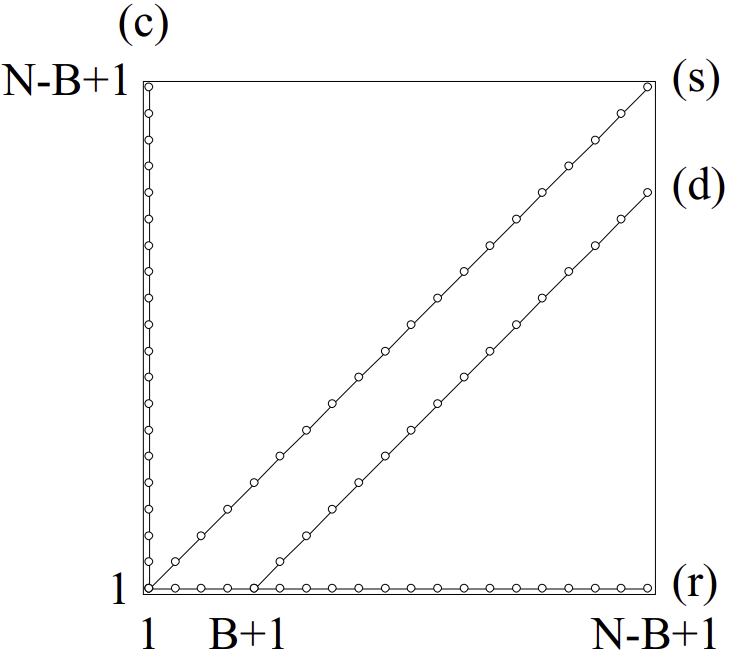
\includegraphics[width=\linewidth, height=0.8\linewidth]{imgs/det_funcs}
				\caption{Функции обнаружения неоднородности. $ B=T $.}\par 
			\end{figure}
		\end{multicols}
	
		{\color{blue} Обозначения функций обнаружения неоднородности:}
		\begin{enumerate}
			\item Строковая: $ d_{n-1}^{(r)} $
			
			\item Столбцовая: $ d_{n-1}^{(c)} $
			
			\item Диагональная: $ d_{n-1}^{(d)} $
			
			\item Симметричная: $ d_{n-1}^{(s)} $
		\end{enumerate}
	\end{frame}

	\begin{frame}
		\frametitle{Часть 1. Сравнение функций обнаружения}
		{\color{blue} Задача:} 
		Сравнить функции обнаружения неоднородности для разных видов разладки.
		
		\bigskip
		{\color{blue} Ряд:}
		$ F_N=(f_1, \dots, f_{N}) $, где $f_n = 
		\begin{cases}
			C_1\sin(2\pi\omega_1n + \phi_1),& n < Q, \\
			C_2\sin(2\pi\omega_2n + \phi_2),& n \geq Q,
		\end{cases}$
		
%		\bigskip
		{\color{blue} Параметры:}
		\begin{enumerate}
			\item $ N = 700 $.
			\item $ Q = 301 $.
			\item $ L = 60 $.
			\item $ B = T = 100 $.
		\end{enumerate}
	
		\bigskip
		
		{\color{blue} Задание неоднородности ряда $ F_N $:}
		\begin{enumerate}
			\item Изменение частоты: $\omega_1 = \frac{1}{10}, \omega_2 = \frac{1}{5}, C_1 = C_2 = 1, \phi_1 = \phi_2 = 0$.
			\item Изменение амплитуды: $ C_1 = 1, C_2 = 2, \omega_1 = \omega_2 = \frac{1}{10}, \phi_1 = \phi_2 = 0 $.
			\item Фазовый сдвиг: $ \phi_1 = 0, \phi_2 = \frac{\pi}{2}, \omega_1 = \omega_2 = \frac{1}{10}, C_1 = C_2 = 1 $.
			\item Выброс: $f_n = 
			\begin{cases}
				C_1\sin(2\pi\omega_1n + \phi_1), & n \neq Q, \\
				10\cdot C_1, & n = Q.
			\end{cases}
			$
		\end{enumerate}
	\end{frame}
	
	\begin{frame}
		\frametitle{Часть 1. Сравнение функций обнаружения}
			\begin{center}
				{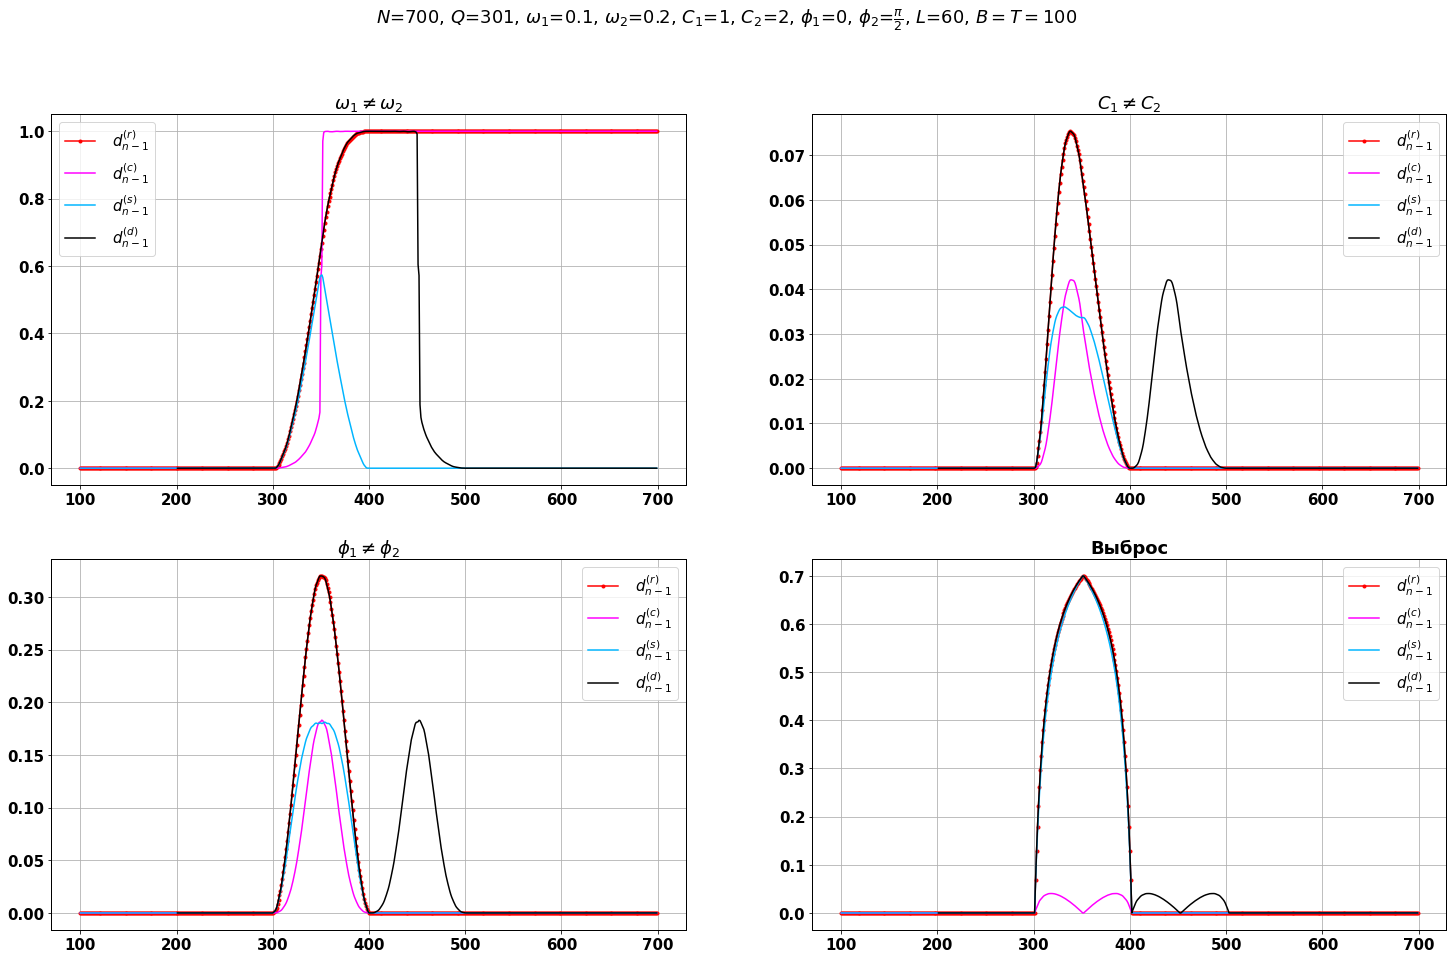
\includegraphics[width=\linewidth]{imgs/detectionTests}}
			\end{center}
			{\color{blue} Вывод:} Лучшие --- \textbf{строковая} $ d_{n-1}^{(r)} $ и \textbf{диагональная} $ d_{n-1}^{(d)} $ функции обнаружения.
	\end{frame}

	\begin{frame}
		\frametitle{Часть 2. Аппроксимация значения индекса неоднородности после переходного интервала}
		{\color{blue} Ряд:}
		$ F_N=(f_1, \dots, f_{N}) $, где $f_n = 
		\begin{cases}
			C_1\sin(2\pi\omega_1n + \phi_1),& n < Q, \\
			C_2\sin(2\pi\omega_2n + \phi_2),& n \geq Q.
		\end{cases}$
	
		\bigskip
		
		{\color{blue} Параметры ряда:} $ \omega_1 \neq \omega_2 $, $ C_1 = C_2 = 1 $.
		
		\bigskip
		{\color{blue} Задача:}
		Аппроксимировать индекс неоднородности $ g(F^{(1)}; F^{(2)}) $, $ F^{(1)} $ лежит до $ Q $, $ F^{(2)} $ после.
		
		\bigskip
		{\color{blue} Результат:}
		\begin{small}
			$$ g_a(\omega_1, \omega_2) = 1 - \frac{\left[ \left(  \frac{\sin(2\pi Lb)}{4\pi b} - \frac{\sin(2\pi La)}{4\pi a}   \right)^2 + \left(  \frac{\cos(2\pi Lb) - 1}{4\pi b} - \frac{\cos(2\pi La) - 1}{4\pi a}  \right)^2 \right]}{\frac{L^2}{4}}, $$
		\end{small}
		
		где $ a = \omega_1 + \omega_2 $, $ b = \omega_1 - \omega_2 $.
		\begin{center}
			{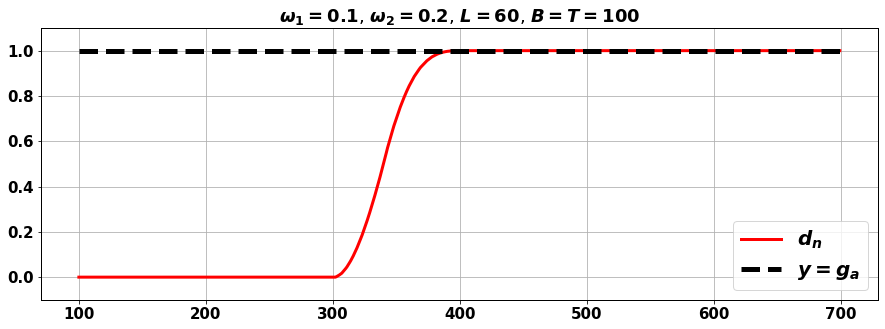
\includegraphics[width=0.7\linewidth]{imgs/example_approx.png}}
			\end{center}
	\end{frame}
	

	\begin{frame}
		\frametitle{Часть 2. Точность аппроксимации}
		\center{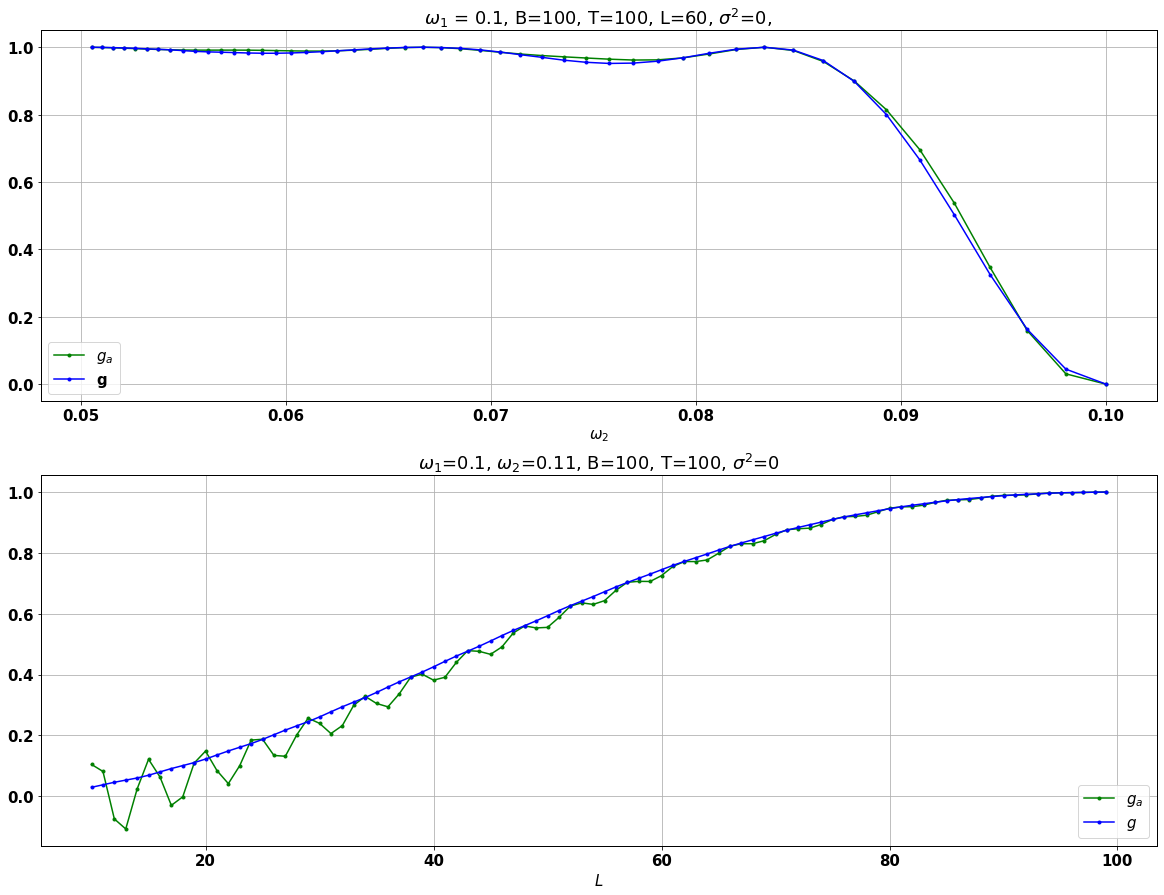
\includegraphics[width=0.9\linewidth]{imgs/approxCorrectness}}
	\end{frame}

	\begin{frame}
		\frametitle{Часть 2. Аппроксимация переходного интервала}
		При достаточно маленьком значении $ L $ по отношению к $ T $ переходный интервал становится линейным.
		
		\begin{figure}[!hhh]
			\center{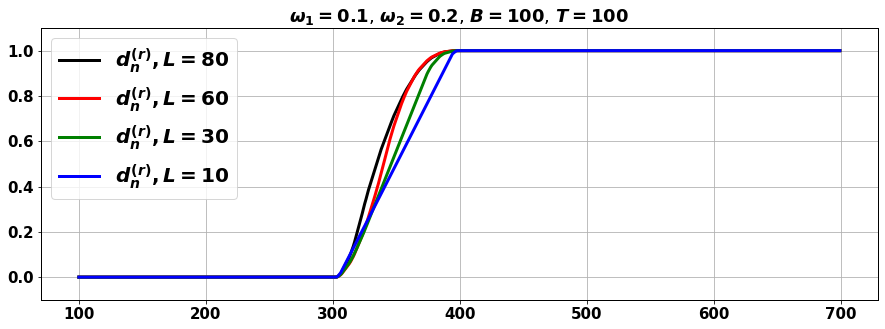
\includegraphics[width=0.9\linewidth]{imgs/row_linear_growth}}
			\caption{Линейность переходного интервала при большом значении $ T-L $.}
			\label{pic:row_linear_growth}
		\end{figure}
	\end{frame}
	
	\begin{frame}
		\frametitle{Часть 3. Система обнаружения момента возмущения}
		{\color{blue} Задача:}
		Обнаружить разладку на интервале от $ Q $ до $ Q + k $, где $ Q $ --- неизвестный момент возмущения, а $ k $ --- максимально допустимое запаздывание.
		
		{\color{blue} Подход:} $ d_{n-1}^{(r)} > \gamma^* $ --- сигнал о моменте возмущения $ \hat{Q}$.
		
		\bigskip
		{\color{blue} Ограничение:} $ \omega_2 > \omega_1 + \Delta_{min} = \omega_{min}$
		
		\bigskip
		Как выбрать $ \gamma^* $? Построить аппроксимацию $ d_{n-1}^{(r)} $ и взять ее значение в точке $ k $.
		
		
		\bigskip
		{\color{blue} Описание системы:}
		\begin{enumerate}
			\item Входные данные: $ F_N $, $ k $, $ \Delta_{min} $.
			\item Результат: $ \hat{Q}$.
		\end{enumerate}
	
		\begin{figure}[!hhh]
			\center{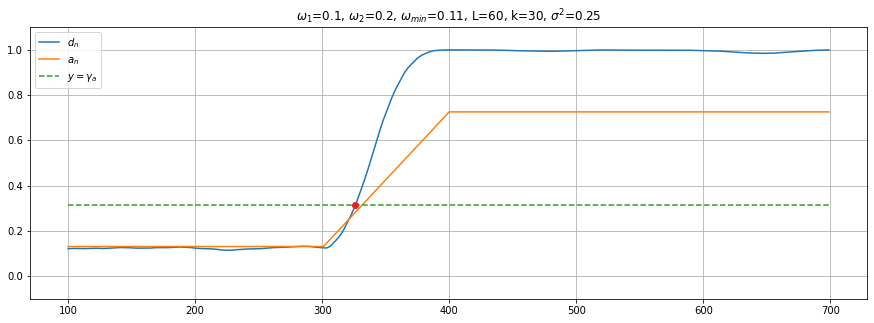
\includegraphics[width=0.9\linewidth]{imgs/example_system_work}}
			\caption{Система. Пример работы.}
			\label{pic:example_system_work}
		\end{figure}
	\end{frame}
	
	\begin{frame}
		\frametitle{Часть 3. Оценка качества системы}
		{\color{blue} Характеристики системы:}
		\begin{itemize}
			\item $ \mathrm{FP}(\gamma^*) $ при $ \hat{Q} < Q $.
			\item $ \mathrm{TP}(\gamma^*) $ при $ \hat{Q} \in [Q, Q+k] $.
			\item $ \mathrm{FN}(\gamma^*) $ при $ \hat{Q} > Q+k $.
		\end{itemize}
		
		\bigskip 
		Промоделируем $ n_{iter}=200 $ раз реализацию шума $ \epsilon $ и на каждой итерации посчитаем характеристики системы. 
		
		\bigskip
		
		{\color{blue} Вероятности обнаружения:}
		
		\begin{itemize}
			\item  $ \mathrm{FPR}(\gamma^*) = \frac{\sum\limits_{i=1}^{n_{iter}}\mathrm{FP}_i(\gamma^*)}{n_{iter}} $.
			\item $ \mathrm{TPR}(\gamma^*) = \frac{\sum\limits_{i=1}^{n_{iter}}\mathrm{TP}_i(\gamma^*)}{n_{iter}} $.
			\item $ \mathrm{FNR}(\gamma^*) = \frac{\sum\limits_{i=1}^{n_{iter}}\mathrm{FN}_i(\gamma^*)}{n_{iter}} $.
		\end{itemize}
	\end{frame}
	
	\begin{frame}
		\frametitle{Часть 3. Оценка системы: $ T - L $}
		\begin{figure}[!hhh]
			\center{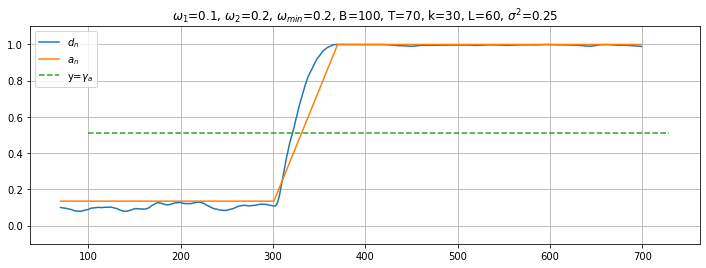
\includegraphics[width=0.9\linewidth]{imgs/system_estimation_one_iter_t=70.png}}
			\caption{Функция обнаружения неоднородности. $ T - L = 10 $.}
			\label{pic:system_estimation_one_iter_t=70}
		\end{figure}
		
		\begin{figure}[!hhh]
			\center{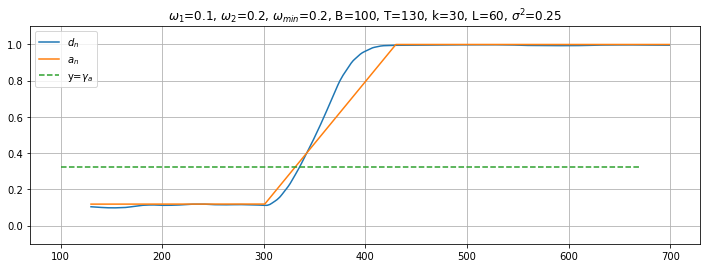
\includegraphics[width=0.9\linewidth]{imgs/system_estimation_one_iter_t=130.png}}
			\caption{Функция обнаружения неоднородности. $ T-L = 70 $.}
			\label{pic:system_estimation_one_iter_t=130}
		\end{figure}
	\end{frame}
	
	\begin{frame}
		\frametitle{Часть 3. Оценка системы: параметр $ T - L $}
		\begin{figure}[!hhh]
			\center{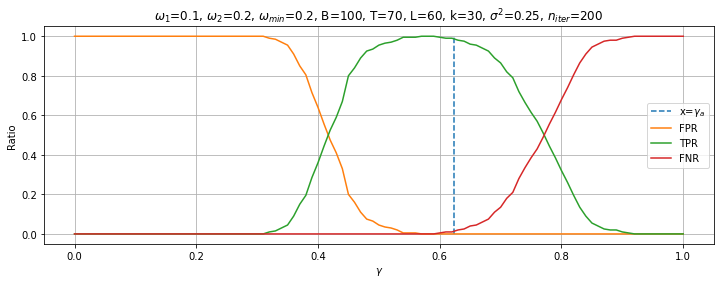
\includegraphics[width=0.9\linewidth]{imgs/system_estimation_t=70.png}}
			\caption{Работы системы. Оценка, $ T - L = 10 $.}
			\label{pic:system_estimation_t=70}
		\end{figure}
		
		\begin{figure}[!hhh]
			\center{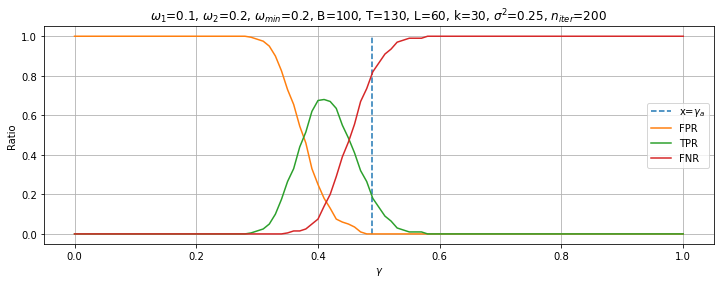
\includegraphics[width=0.9\linewidth]{imgs/system_estimation_t=130.png}}
			\caption{Работы системы. Оценка, $ T - L = 70 $.}
			\label{pic:system_estimation_t=130}
		\end{figure}
	\end{frame}
	
	
	
%	\begin{frame}
%		\frametitle{Тестирование системы}
%		\begin{table}[!hhh]
%			\center
%			\caption{Результаты тестирования модели, $ N = 800, Q=301, k=15 $.}
%			\begin{tabular}{cccccccccc}
%				\toprule
%				$ \omega_1 $ & $ \omega_2 $ & $ \Delta_{min} $ & $ \sigma $ &    $ B $ &   $ T $ &   $ L $ &    $ FPR $ &    $ TPR $ &    $ FNR $ \\
%				\midrule
%				1/10 &     1/3 &        0.02 &     0.2 & 133 & 79 & 71 & 0.000 & 1.0 & 0.000 \\
%				1/10 &     1/3 &        0.02 &     0.3 & 133 & 79 & 71 & 0.000 & 0.995 & 0.005 \\
%				1/10 &     1/3 &        0.02 &     0.4 & 133 & 79 & 71 & 0.000 & 0.895 & 0.105 \\
%				1/10 &     1/3 &        0.02 &     0.5 & 133 & 79 & 71 & 0.040 & 0.745 & 0.215 \\
%				\hline
%				1/10 &     1/4 &        0.02 &     0.2 & 133 & 79 & 71 & 0.000 & 1.0 & 0.000 \\
%				1/10 &     1/4 &        0.02 &     0.3 & 133 & 79 & 71 & 0.000 & 0.980 & 0.020 \\
%				1/10 &     1/4 &        0.02 &     0.4 & 133 & 79 & 71 & 0.000 & 0.870 & 0.130 \\
%				1/10 &     1/4 &        0.02 &     0.5 & 133 & 79 & 71 & 0.040 & 0.745 & 0.215 \\
%				\hline
%				1/10 &     1/5 &        0.02 &     0.2 & 133 & 79 & 71 & 0.000 & 1.0 & 0.000 \\
%				1/10 &     1/5 &        0.02 &     0.3 & 133 & 79 & 71 & 0.000 & 0.980 & 0.020 \\
%				1/10 &     1/5 &        0.02 &     0.4 & 133 & 79 & 71 & 0.000 & 0.855 & 0.145 \\
%				1/10 &     1/5 &        0.02 &     0.5 & 133 & 79 & 71 & 0.040 & 0.720 & 0.240 \\
%				\hline
%				1/10 &     1/6 &        0.02 &     0.2 & 133 & 79 & 71 & 0.000 & 1.0 & 0.000 \\
%				1/10 &     1/6 &        0.02 &     0.3 & 133 & 79 & 71 & 0.000 & 0.995 & 0.005 \\
%				1/10 &     1/6 &        0.02 &     0.4 & 133 & 79 & 71 & 0.000 & 0.925 & 0.075 \\
%				1/10 &     1/6 &        0.02 &     0.5 & 133 & 79 & 71 & 0.040 & 0.820 & 0.140 \\
%				\bottomrule
%			\end{tabular}
%			\label{tab:simplified_system_results_k=15_1}
%		\end{table}
%	\end{frame}	
%	
%	\begin{frame}
%		\frametitle{Тестирование системы}
%		\begin{table}[!hhh]
%			\center
%			\caption{Результаты тестирования модели, $ N = 800, Q=301, k=15 $.}
%			\begin{tabular}{cccccccccc}
%				\toprule
%				$ \omega_1 $ & $ \omega_2 $ & $ \Delta_{min} $ & $ \sigma $ &    $ B $ &   $ T $ &   $ L $ &    $ FPR $ &    $ TPR $ &    $ FNR $ \\
%				\midrule
%				1/10&     1/7 &        0.02 &     0.0 & 133 & 79 & 71 & 0.000 & 0.000 & 1.000 \\
%				1/10&     1/7 &        0.02 &     0.1 & 133 & 79 & 71 & 0.000 & 0.250 & 0.750 \\
%				1/10&     1/7 &        0.02 &     0.2 & 133 & 79 & 71 & 0.000 & 0.335 & 0.665 \\
%				1/10&     1/7 &        0.02 &     0.3 & 133 & 79 & 71 & 0.000 & 0.325 & 0.675 \\
%				1/10&     1/7 &        0.02 &     0.4 & 133 & 79 & 71 & 0.000 & 0.380 & 0.620 \\
%				1/10&     1/7 &        0.02 &     0.5 & 133 & 79 & 71 & 0.040 & 0.340 & 0.660 \\
%				\hline
%				1/10&     1/8 &        0.02 &     0.2 & 133 & 79 & 71 & 0.000 & 1.0 & 0.000 \\
%				1/10&     1/8 &        0.02 &     0.3 & 133 & 79 & 71 & 0.000 & 1.0 & 0.000 \\
%				1/10&     1/8 &        0.02 &     0.4 & 133 & 79 & 71 & 0.000 & 0.995 & 0.005 \\
%				1/10&     1/8 &        0.02 &     0.5 & 133 & 79 & 71 & 0.040 & 0.920 & 0.040 \\
%				\hline
%				1/10 &     1/9 &        0.02 &     0.4 & 133 & 79 & 71 & 0.000 & 1.0 & 0.000 \\
%				1/10 &     1/9 &        0.02 &     0.5 & 133 & 79 & 71 & 0.050 & 0.950 & 0.000 \\
%				\bottomrule
%			\end{tabular}
%			\label{tab:simplified_system_results_k=15_2}
%		\end{table}
%	
%	\end{frame}	
	
	\begin{frame}
		\frametitle{Часть 3. Проблемы}
		{\color{blue} Параметры тестирования:} $ N = 800, Q=301, \omega_1=\frac{1}{10} , \Delta_{min}=\frac{1}{50}, \sigma=0.5, B=133, T=79, L=71, C_1=C_2=1$
		
		\bigskip
		
		\begin{table}[!hhh]
			\center
			\caption{Результаты тестирования.}
			\begin{minipage}{.5\linewidth}
				\caption{$ k=30 $}
				\centering
				\begin{tabular}{cccc}
					\toprule
					$ \omega_2 $ & $ FPR $ &    $ TPR $ &    $ FNR $ \\
					1/3 &  0.0 &   0.99 &   0.01 \\
					1/4 &  0.0 &   0.98 &   0.02 \\
					1/5 &  0.0 &   0.99 &   0.01 \\
					1/6 &  0.0 &  0.995 &  0.005 \\				
					1/7 &  0.0 &  0.945 &  0.055 \\
					1/8 &  0.0 &  0.855 &  0.145 \\
					1/9 &  0.0 &    1.0 &    0.0 \\
					\bottomrule
				\end{tabular}
			\end{minipage}%
			\begin{minipage}{.5\linewidth}
				\caption{$ k=15 $}
				\centering
				\begin{tabular}{cccc}
					\toprule
					$ \omega_2 $ & $ FPR $ &    $ TPR $ &    $ FNR $ \\
					1/3 &  0.040 & 0.745 & 0.215  \\
					1/4 &  0.040 & 0.745 & 0.215 \\
					1/5 &  0.040 & 0.720 & 0.240 \\
					1/6 &  0.040 & 0.820 & 0.140 \\				
					1/7 &  0.040 & 0.340 & 0.660 \\
					1/8 &  0.040 & 0.920 & 0.040  \\
					1/9 &  0.050 & 0.950 & 0.000  \\
					\bottomrule
				\end{tabular}
			\end{minipage}%
		\end{table}
	
	
		\bigskip
		
		{\color{blue} Выводы:} При большом $ k $ система работает хорошо, но аппроксимация нуждается в доработке.
	
	\end{frame}	
	

\end{document}
